\documentclass[aspectratio=169]{beamer}

\usepackage[UTF8,noindent]{ctexcap}
\usepackage{amsmath}
\usepackage{color}

\usepackage[utf8]{inputenc}
\usepackage{bookman}
\usepackage{tikz}
\usetikzlibrary{shapes.geometric}

\usetikzlibrary{math,calc}

\usepackage{ctex}
\usepackage{multicol}
\usetikzlibrary{mindmap,trees}
\usepackage{verbatim}
%\usepackage[text={176mm,250mm},left=1cm,right=1cm,vmarginratio=1:1]{geometry}


\usetheme{opensuse}

\title{基于图形计算器}
\subtitle{开展对正整数立方和的探究性学习}
\author{徐希来}
\date{June 12th 2019}
\newcommand{\authortitle}{}
\newcommand{\organization}{上海市大同中学}
\newcommand{\event}{第十七届“TI手持教育技术与中学数学教学改革”年会}
\newcommand{\location}{市教委教研室(陕西北路500号)}

\begin{document}
 
\frame{\titlepage}

 \begin{frame}
 \frametitle{目录}
 \begin{multicols}{2}
 	\tableofcontents%[hideallsubsections]%[part=1,pausesections]
 \end{multicols}

\end{frame}

\section{问题背景}

\section{问题解决}

\subsection{1.在数的阵列队形中摸索规律}
      \begin{frame}
     \frametitle{1.在数的阵列队形中摸索规律}
     \colorbox{green!70!yellow}{$ 1^3 $}  
     \\ \vspace{1em}
     \colorbox{green!70!blue}{$ 2^3 $}    
     \\ \vspace{1em}
     \colorbox{green!50!blue}{$ 3^3 $}     
     \\  \vspace{1em}
     \colorbox{green!50!black}{$ 4^3 $}    
     \\
     \end{frame}

      \begin{frame}
     \frametitle{1.在数的阵列队形中摸索规律}
     \colorbox{green!70!yellow}{$ 1^3 $}   $ \longrightarrow $   \colorbox{green!70!yellow}{$ 1 \times 1 $}  
     \\ \vspace{1em}
     \colorbox{green!70!blue}{$ 2^3 $}    $ \longrightarrow $   \colorbox{green!70!blue}{$ 2 \times 4 $}   
     \\ \vspace{1em}
     \colorbox{green!50!blue}{$ 3^3 $}     $ \longrightarrow $   \colorbox{green!50!blue}{$ 3 \times 9 $}   
     \\  \vspace{1em}
     \colorbox{green!50!black}{$ 4^3 $}    $ \longrightarrow $  \colorbox{green!50!black}{$ 4 \times 16 $}  
     \\
     
 \end{frame}

    \begin{frame}
    \frametitle{1.在数的阵列队形中摸索规律}
    \colorbox{green!70!yellow}{$ 1^3 $}   $ \longrightarrow $   \colorbox{green!70!yellow}{$ 1 \times 1 $}  
    \hspace{2.1cm}  \colorbox{green!70!yellow}{1}
     \\ \vspace{1em}
     \colorbox{green!70!blue}{$ 2^3 $}    $ \longrightarrow $   \colorbox{green!70!blue}{$ 2 \times 4 $}   
      \hspace{2.1cm}    \colorbox{green!70!blue}{3}  \hspace{1cm}   \colorbox{green!70!blue}{5} 
     \\ \vspace{1em}
      \colorbox{green!50!blue}{$ 3^3 $}     $ \longrightarrow $   \colorbox{green!50!blue}{$ 3 \times 9 $}   
       \hspace{2.1cm}    \colorbox{green!50!blue}{7}  
       \hspace{1cm} \colorbox{green!50!blue}{9} 
        \hspace{1cm} \colorbox{green!50!blue}{11} 
      \\  \vspace{1em}
       \colorbox{green!50!black}{$ 4^3 $}    $ \longrightarrow $  \colorbox{green!50!black}{$ 4 \times 16 $}  
        \hspace{1.9cm}   \colorbox{green!50!black}{13} 
         \hspace{0.85cm} \colorbox{green!50!black}{15} 
         \hspace{0.85cm} \colorbox{green!50!black}{17} 
          \hspace{0.85cm} \colorbox{green!50!black}{19} 
        \\
    
    \end{frame}
\subsubsection{(1)三角形数阵}
       \begin{frame}
      \frametitle{(1)三角形数阵}
      \begin{columns}
      	\column{0.48\textwidth}
      	\includegraphics[scale=0.3]{三角形数阵.jpg}
      	\vspace{2cm}
      	\column{0.48\textwidth}
      	\includegraphics[scale=0.3]{三角形数阵和式.jpg}
      	\vspace{2cm}
      \end{columns}      
  \end{frame}
     
       \begin{frame}
     \frametitle{(1)三角形数阵}
     \begin{columns}
     	\column{0.48\textwidth}
     	\includegraphics[scale=0.255]{奇数和拼图.jpg}\\
         \footnotesize \phantom{从1开始的连续$ \frac{n\left( n+1\right) }{2} $个奇数的和}\\
        \vspace{2cm}
     	\column{0.48\textwidth}
     	\includegraphics[scale=0.3]{奇数和计算.jpg}
     	 \footnotesize 从1开始的连续$ \frac{n\left( n+1\right) }{2} $个奇数的和\\
     	\vspace{2cm}
     \end{columns}      
 \end{frame}

\subsubsection{(2)正方形数阵}
        \begin{frame}
       \frametitle{(2)正方形数阵}
       \begin{columns}
       	\column{0.48\textwidth}
       	\includegraphics[scale=0.255]{正方形数阵.jpg}
       	\vspace{2cm}
       	\column{0.48\textwidth}
       	\includegraphics[scale=0.3]{正方形数阵和式.jpg}
       	\vspace{2cm}
       \end{columns}      
   \end{frame}

 
\subsubsection{(3)矩形数阵}
       \begin{frame}
      \frametitle{(3)矩形数阵}
      \begin{columns}
      	\column{0.48\textwidth}
      	\includegraphics[scale=0.3]{矩形数阵.jpg}
      	\vspace{2cm}
      	\column{0.48\textwidth}
      	\includegraphics[scale=0.3]{矩形数阵和式.jpg}
      	\vspace{2cm}
      \end{columns}      
  \end{frame}

\subsubsection{(4)差分表}

\begin{frame}
\frametitle{(4)差分表}

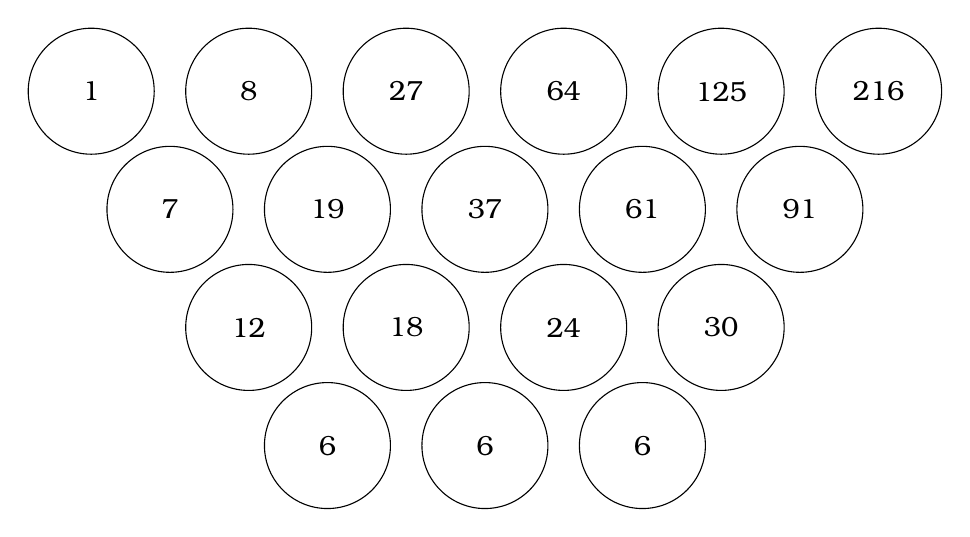
\begin{tikzpicture}[scale=1]

\foreach \x in {0,2,4,6,8,10}  {
	\draw (\x,0) circle (0.8);
} 
\node () at (0,0) {1};   
\node () at (2,0) {8};
\node () at (4,0) {27};
\node () at (6,0) {64};
\node () at (8,0) {125};
\node () at (10,0) {216};

\foreach \x in {1,3,5,7,9}  {
	\draw (\x,-1.5) circle (0.8);
} 
\node () at (1,-1.5) {7};
\node () at (3,-1.5) {19};
\node () at (5,-1.5) {37};
\node () at (7,-1.5) {61};
\node () at (9,-1.5) {91};


\foreach \x in {2,4,6,8}  {
	\draw (\x,-3) circle (0.8);
} 
\node () at (2,-3) {12};
\node () at (4,-3) {18};
\node () at (6,-3) {24};
\node () at (8,-3) {30};


\foreach \x in {3,5,7}  {
	\draw (\x,-4.5) circle (0.8);
} 
\node () at (3,-4.5) {6};
\node () at (5,-4.5) {6};
\node () at (7,-4.5) {6};

\end{tikzpicture}
\end{frame}


       \begin{frame}
       \frametitle{(4)差分表}
        
       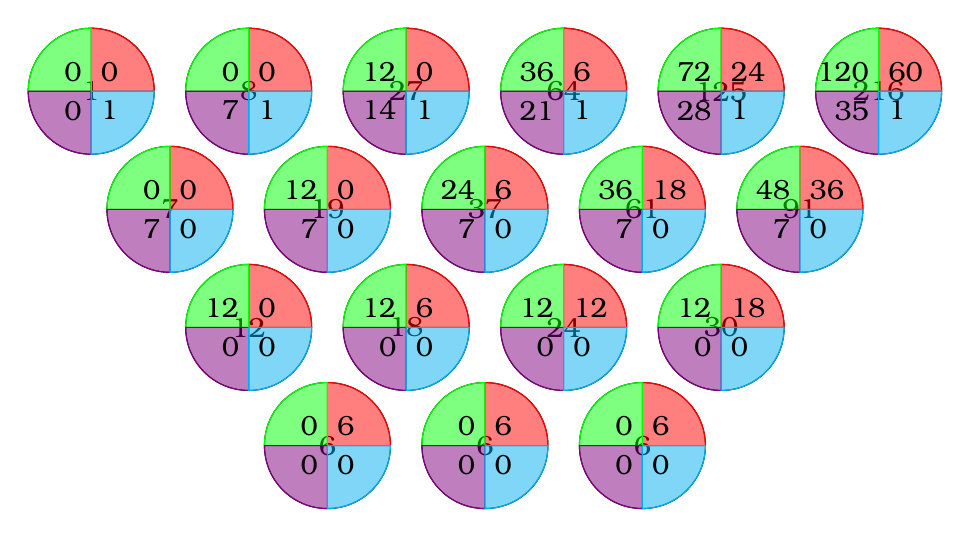
\begin{tikzpicture}[scale=1]
       
         \foreach \x in {0,2,4,6,8,10}  {
         \draw (\x,0) circle (0.8);
         } 
         \node () at (0,0) {1};   
         \node () at (2,0) {8};
         \node () at (4,0) {27};
         \node () at (6,0) {64};
         \node () at (8,0) {125};
         \node () at (10,0) {216};
         
        \foreach \x in {1,3,5,7,9}  {
       	\draw (\x,-1.5) circle (0.8);
        } 
        \node () at (1,-1.5) {7};
        \node () at (3,-1.5) {19};
        \node () at (5,-1.5) {37};
        \node () at (7,-1.5) {61};
        \node () at (9,-1.5) {91};
        
        
         \foreach \x in {2,4,6,8}  {
        	\draw (\x,-3) circle (0.8);
        } 
        \node () at (2,-3) {12};
        \node () at (4,-3) {18};
        \node () at (6,-3) {24};
        \node () at (8,-3) {30};
        
        
         \foreach \x in {3,5,7}  {
        	\draw (\x,-4.5) circle (0.8);
        } 
        \node () at (3,-4.5) {6};
        \node () at (5,-4.5) {6};
        \node () at (7,-4.5) {6};
         
    
%第一象限    
       	 \foreach \x in {0,2,4,6,8,10}  {
       	\filldraw[fill=red,fill opacity=0.5,draw=red] (\x,0) -- (\x+0.8,0)
       	arc [start angle=0, end angle=90, radius=0.8]--(\x,0);
       }
        	\node () at (0,0) [above right]{0};
            \node () at (2,0) [above right]{0};
            \node () at (4,0) [above right]{0};
            \node () at (6,0) [above right]{6};
            \node () at (8,0) [above right]{24};
            \node () at (10,0) [above right]{60};
       	
       
       	 \foreach \x in {1,3,5,7,9}  {
       	\filldraw[fill=red,fill opacity=0.5,draw=red] (\x,-1.5) -- (\x+0.8,-1.5)
       	arc [start angle=0, end angle=90, radius=0.8]--(\x,-1.5);
       }
       \node () at (1,-1.5) [above right]{0};
       \node () at (3,-1.5) [above right]{0};
       \node () at (5,-1.5) [above right]{6};
       \node () at (7,-1.5) [above right]{18};
       \node () at (9,-1.5) [above right]{36};
  
       	 \foreach \x in {2,4,6,8}  {
       	\filldraw[fill=red,fill opacity=0.5,draw=red] (\x,-3) -- (\x+0.8,-3)
       	arc [start angle=0, end angle=90, radius=0.8]--(\x,-3);
       }
       \node () at (2,-3) [above right]{0};
       \node () at (4,-3) [above right]{6};
       \node () at (6,-3) [above right]{12};
       \node () at (8,-3) [above right]{18};
     
     	 \foreach \x in {3,5,7}  {
     	\filldraw[fill=red,fill opacity=0.5,draw=red] (\x,-4.5) -- (\x+0.8,-4.5)
     	arc [start angle=0, end angle=90, radius=0.8]--(\x,-4.5);
     	\node () at (\x,-4.5) [above right]{6};
     }

     
%第二象限       	
       	\foreach \x in {0,2,4,6,8,10}  {
       	\filldraw[fill=green,fill opacity=0.5,draw=green] (\x,0) -- (\x-0.8,0)
       	arc [start angle=180, end angle=90, radius=0.8]--(\x,0);
       	}
   
            \node () at (0,0) [above left]{0};
            \node () at (2,0) [above left]{0};      
            \node () at (4,0) [above left]{12};  
            \node () at (6,0) [above left]{36};
            \node () at (8,0) [above left]{72};
            \node () at (10,0) [above left]{120};
            
         \foreach \x in {1,3,5,7,9}  {
         	\filldraw[fill=green,fill opacity=0.5,draw=green] (\x,-1.5) -- (\x-0.8,-1.5)
         	arc [start angle=180, end angle=90, radius=0.8]--(\x,-1.5);
         }
         
         \node () at (1,-1.5) [above left]{0};
         \node () at (3,-1.5) [above left]{12};      
         \node () at (5,-1.5) [above left]{24};  
         \node () at (7,-1.5) [above left]{36};
         \node () at (9,-1.5) [above left]{48};
     
         
         	\foreach \x in {2,4,6,8}  {
         	\filldraw[fill=green,fill opacity=0.5,draw=green] (\x,-3) -- (\x-0.8,-3)
         	arc [start angle=180, end angle=90, radius=0.8]--(\x,-3);
         	 \node () at (\x,-3) [above left]{12};   
         }
         
            \foreach \x in {3,5,7}  {
           	\filldraw[fill=green,fill opacity=0.5,draw=green] (\x,-4.5) -- (\x-0.8,-4.5)
           	arc [start angle=180, end angle=90, radius=0.8]--(\x,-4.5);
           	  \node () at (\x,-4.5) [above left]{0};     
           }
           
  %第三象限         
            
        \foreach \x in {0,2,4,6,8,10}  {  
       	\filldraw[fill=violet,fill opacity=0.5,draw=violet] (\x,0) -- (\x-0.8,0)
       	arc [start angle=180, end angle=270, radius=0.8]--(\x,0);
       }
       	     \node () at (0,0) [below left]{0};
       	     \node () at (2,0) [below left]{7};
       	     \node () at (4,0) [below left]{14};
       	     \node () at (6,0) [below left]{21};
       	     \node () at (8,0) [below left]{28};
       	     \node () at (10,0) [below left]{35};
       	     
       	 \foreach \x in {1,3,5,7,9}  {  
       		\filldraw[fill=violet,fill opacity=0.5,draw=violet] (\x,-1.5) -- (\x-0.8,-1.5)
       		arc [start angle=180, end angle=270, radius=0.8]--(\x,-1.5);
       		\node () at (\x,-1.5) [below left]{7};
       	}
       
       
        \foreach \x in {2,4,6,8}  {  
       	\filldraw[fill=violet,fill opacity=0.5,draw=violet] (\x,-3) -- (\x-0.8,-3)
       	arc [start angle=180, end angle=270, radius=0.8]--(\x,-3); \node () at (\x,-3) [below left]{0};
       }
      
      
          \foreach \x in {3,5,7}  {  
         	\filldraw[fill=violet,fill opacity=0.5,draw=violet] (\x,-4.5) -- (\x-0.8,-4.5)
         	arc [start angle=180, end angle=270, radius=0.8]--(\x,-4.5);
         	\node () at (\x,-4.5) [below left]{0};
         }
        
%第四象限       	
       	\foreach \x in {0,2,4,6,8,10}  {
       	\filldraw[fill=cyan,fill opacity=0.5,draw=cyan] (\x,0) -- (\x+0.8,0)
       	arc [start angle=0, end angle=-90, radius=0.8]--(\x,0);
        \node () at (\x,0)[below right] {1};
        }
       	    
       	   \foreach \x in {1,3,5,7,9}  {
       	   	\filldraw[fill=cyan,fill opacity=0.5,draw=cyan] (\x,-1.5) -- (\x+0.8,-1.5)
       	   	arc [start angle=0, end angle=-90, radius=0.8]--(\x,-1.5);
       	   	\node () at (\x,-1.5)[below right] {0};
       	   }  
       	
       	
       		\foreach \x in {2,4,6,8}  {
       		\filldraw[fill=cyan,fill opacity=0.5,draw=cyan] (\x,-3 )-- (\x+0.8,-3)
       		arc [start angle=0, end angle=-90, radius=0.8]--(\x,-3);
       		\node () at (\x,-3)[below right] {0};
       	}
       
       \foreach \x in {3,5,7}  {
       	\filldraw[fill=cyan,fill opacity=0.5,draw=cyan] (\x,-4.5) -- (\x+0.8,-4.5)
       	arc [start angle=0, end angle=-90, radius=0.8]--(\x,-4.5);
       	\node () at (\x,-4.5)[below right] {0};
       }  
       
       \end{tikzpicture}
       \end{frame}
   
%第一张差分表
      \begin{frame}
     \frametitle{(4)差分表}
     
     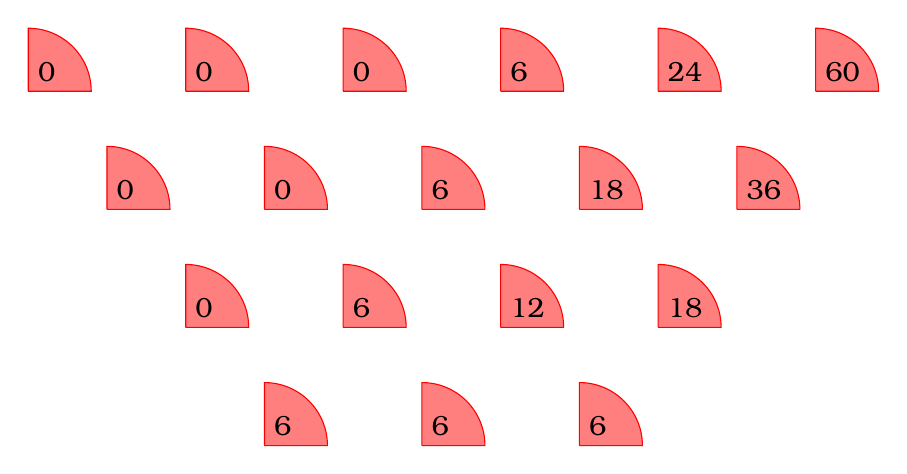
\begin{tikzpicture}[scale=1]
     %第一象限    
     \foreach \x in {0,2,4,6,8,10}  {
     	\filldraw[fill=red,fill opacity=0.5,draw=red] (\x,0) -- (\x+0.8,0)
     	arc [start angle=0, end angle=90, radius=0.8]--(\x,0);
     }
     \node () at (0,0) [above right]{0};
     \node () at (2,0) [above right]{0};
     \node () at (4,0) [above right]{0};
     \node () at (6,0) [above right]{6};
     \node () at (8,0) [above right]{24};
     \node () at (10,0) [above right]{60};
     
     
     \foreach \x in {1,3,5,7,9}  {
     	\filldraw[fill=red,fill opacity=0.5,draw=red] (\x,-1.5) -- (\x+0.8,-1.5)
     	arc [start angle=0, end angle=90, radius=0.8]--(\x,-1.5);
     }
     \node () at (1,-1.5) [above right]{0};
     \node () at (3,-1.5) [above right]{0};
     \node () at (5,-1.5) [above right]{6};
     \node () at (7,-1.5) [above right]{18};
     \node () at (9,-1.5) [above right]{36};
     
     \foreach \x in {2,4,6,8}  {
     	\filldraw[fill=red,fill opacity=0.5,draw=red] (\x,-3) -- (\x+0.8,-3)
     	arc [start angle=0, end angle=90, radius=0.8]--(\x,-3);
     }
     \node () at (2,-3) [above right]{0};
     \node () at (4,-3) [above right]{6};
     \node () at (6,-3) [above right]{12};
     \node () at (8,-3) [above right]{18};
     
     \foreach \x in {3,5,7}  {
     	\filldraw[fill=red,fill opacity=0.5,draw=red] (\x,-4.5) -- (\x+0.8,-4.5)
     	arc [start angle=0, end angle=90, radius=0.8]--(\x,-4.5);
     	\node () at (\x,-4.5) [above right]{6};
     }
      
     \end{tikzpicture}
 \end{frame}



     \begin{frame}
   \frametitle{(4)差分表}
  
   	        \begin{tikzpicture}[scale=0.65]
   	       
   	       %第一象限    
   	       {\footnotesize 
   	       	\foreach \x in {0,2,4,6,8,10}  {
   	       		\filldraw[fill=red,fill opacity=0.5,draw=red] (\x,0) -- (\x+0.8,0)
   	       		arc [start angle=0, end angle=90, radius=0.8]--(\x,0);
   	       	}
   	       	\node () at (0,0) [above right]{0};
   	       	\node () at (2,0) [above right]{0};
   	       	\node () at (4,0) [above right]{0};
   	       	\node () at (6,0) [above right]{6};
   	       	\node () at (8,0) [above right]{24};
   	       	\node () at (10,0) [above right]{60};
   	       	
   	       	
   	       	\foreach \x in {1,3,5,7,9}  {
   	       		\filldraw[fill=red,fill opacity=0.5,draw=red] (\x,-1.5) -- (\x+0.8,-1.5)
   	       		arc [start angle=0, end angle=90, radius=0.8]--(\x,-1.5);
   	       	}
   	       	\node () at (1,-1.5) [above right]{0};
   	       	\node () at (3,-1.5) [above right]{0};
   	       	\node () at (5,-1.5) [above right]{6};
   	       	\node () at (7,-1.5) [above right]{18};
   	       	\node () at (9,-1.5) [above right]{36};
   	       	
   	       	\foreach \x in {2,4,6,8}  {
   	       		\filldraw[fill=red,fill opacity=0.5,draw=red] (\x,-3) -- (\x+0.8,-3)
   	       		arc [start angle=0, end angle=90, radius=0.8]--(\x,-3);
   	       	}
   	       	\node () at (2,-3) [above right]{0};
   	       	\node () at (4,-3) [above right]{6};
   	       	\node () at (6,-3) [above right]{12};
   	       	\node () at (8,-3) [above right]{18};
   	       	
   	       	\foreach \x in {3,5,7}  {
   	       		\filldraw[fill=red,fill opacity=0.5,draw=red] (\x,-4.5) -- (\x+0.8,-4.5)
   	       		arc [start angle=0, end angle=90, radius=0.8]--(\x,-4.5);
   	       		\node () at (\x,-4.5) [above right]{6};
   	       	}
   	        
          
             
            	\foreach \x in {12,14,16,18,20,22}  {
            		\filldraw[fill=red,fill opacity=0.5,draw=red] (\x,0) -- (\x+0.8,0)
            		arc [start angle=0, end angle=90, radius=0.8]--(\x,0);
            	}
            	\node () at (12,0) [above right]{0};
            	\node () at (14,0) [above right]{0};
            	\node () at (16,0) [above right]{0};
            	\node () at (18,0) [above right]{1};
            	\node () at (20,0) [above right]{4};
            	\node () at (22,0) [above right]{10};
            	
            	
            	\foreach \x in {13,15,17,19,21}  {
            		\filldraw[fill=red,fill opacity=0.5,draw=red] (\x,-1.5) -- (\x+0.8,-1.5)
            		arc [start angle=0, end angle=90, radius=0.8]--(\x,-1.5);
            	}
            	\node () at (13,-1.5) [above right]{0};
            	\node () at (15,-1.5) [above right]{0};
            	\node () at (17,-1.5) [above right]{1};
            	\node () at (19,-1.5) [above right]{3};
            	\node () at (21,-1.5) [above right]{6};
            	
            	\foreach \x in {14,16,18,20}  {
            		\filldraw[fill=red,fill opacity=0.5,draw=red] (\x,-3) -- (\x+0.8,-3)
            		arc [start angle=0, end angle=90, radius=0.8]--(\x,-3);
            	}
            	\node () at (14,-3) [above right]{0};
            	\node () at (16,-3) [above right]{1};
            	\node () at (18,-3) [above right]{2};
            	\node () at (20,-3) [above right]{3};
            	
            	\foreach \x in {15,17,19}  {
            		\filldraw[fill=red,fill opacity=0.5,draw=red] (\x,-4.5) -- (\x+0.8,-4.5)
            		arc [start angle=0, end angle=90, radius=0.8]--(\x,-4.5);
            		\node () at (\x,-4.5) [above right]{1};
            	}
            \node () at (5,-6) {{\Huge $ \times 1 $}};
            \node () at (17,-6) {{\Huge $ \times 6 $}};
            \node () at (11,-5.5) {{\Large 分拆}};
               }
   	       	 \draw [->,line width=1pt](7,-6) --(15,-6);      
   	       \end{tikzpicture}

\end{frame}
       
%第二张差分表
       
        \begin{frame}
       \frametitle{(4)差分表}
       
       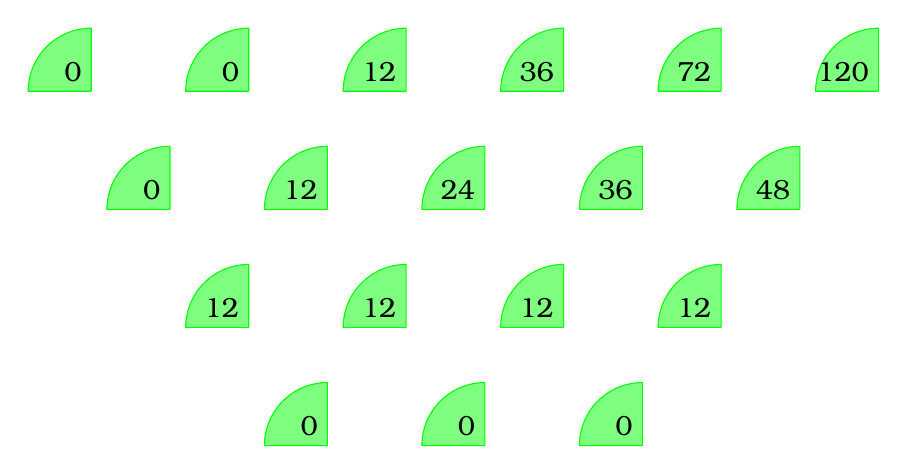
\begin{tikzpicture}[scale=1]
       
      
       %第二象限       	
       \foreach \x in {0,2,4,6,8,10}  {
       	\filldraw[fill=green,fill opacity=0.5,draw=green] (\x,0) -- (\x-0.8,0)
       	arc [start angle=180, end angle=90, radius=0.8]--(\x,0);
       }
       
       \node () at (0,0) [above left]{0};
       \node () at (2,0) [above left]{0};      
       \node () at (4,0) [above left]{12};  
       \node () at (6,0) [above left]{36};
       \node () at (8,0) [above left]{72};
       \node () at (10,0) [above left]{120};
       
       \foreach \x in {1,3,5,7,9}  {
       	\filldraw[fill=green,fill opacity=0.5,draw=green] (\x,-1.5) -- (\x-0.8,-1.5)
       	arc [start angle=180, end angle=90, radius=0.8]--(\x,-1.5);
       }
       
       \node () at (1,-1.5) [above left]{0};
       \node () at (3,-1.5) [above left]{12};      
       \node () at (5,-1.5) [above left]{24};  
       \node () at (7,-1.5) [above left]{36};
       \node () at (9,-1.5) [above left]{48};
       
       
       \foreach \x in {2,4,6,8}  {
       	\filldraw[fill=green,fill opacity=0.5,draw=green] (\x,-3) -- (\x-0.8,-3)
       	arc [start angle=180, end angle=90, radius=0.8]--(\x,-3);
       	\node () at (\x,-3) [above left]{12};   
       }
       
       \foreach \x in {3,5,7}  {
       	\filldraw[fill=green,fill opacity=0.5,draw=green] (\x,-4.5) -- (\x-0.8,-4.5)
       	arc [start angle=180, end angle=90, radius=0.8]--(\x,-4.5);
       	\node () at (\x,-4.5) [above left]{0};     
       }
       
       \end{tikzpicture}
   \end{frame}
       
       
         
       \begin{frame}
       \frametitle{(4)差分表}
       
       \begin{tikzpicture}[scale=0.65]
       
       %第二象限
       {\footnotesize        	
       \foreach \x in {0,2,4,6,8,10}  {
       	\filldraw[fill=green,fill opacity=0.5,draw=green] (\x,0) -- (\x-0.8,0)
       	arc [start angle=180, end angle=90, radius=0.8]--(\x,0);
       }
       
       \node () at (0,0) [above left]{0};
       \node () at (2,0) [above left]{0};      
       \node () at (4,0) [above left]{12};  
       \node () at (6,0) [above left]{36};
       \node () at (8,0) [above left]{72};
       \node () at (10,0) [above left]{120};
       
       \foreach \x in {1,3,5,7,9}  {
       	\filldraw[fill=green,fill opacity=0.5,draw=green] (\x,-1.5) -- (\x-0.8,-1.5)
       	arc [start angle=180, end angle=90, radius=0.8]--(\x,-1.5);
       }
       
       \node () at (1,-1.5) [above left]{0};
       \node () at (3,-1.5) [above left]{12};      
       \node () at (5,-1.5) [above left]{24};  
       \node () at (7,-1.5) [above left]{36};
       \node () at (9,-1.5) [above left]{48};
       
       
       \foreach \x in {2,4,6,8}  {
       	\filldraw[fill=green,fill opacity=0.5,draw=green] (\x,-3) -- (\x-0.8,-3)
       	arc [start angle=180, end angle=90, radius=0.8]--(\x,-3);
       	\node () at (\x,-3) [above left]{12};   
       }
       
       \foreach \x in {3,5,7}  {
       	\filldraw[fill=green,fill opacity=0.5,draw=green] (\x,-4.5) -- (\x-0.8,-4.5)
       	arc [start angle=180, end angle=90, radius=0.8]--(\x,-4.5);
       	\node () at (\x,-4.5) [above left]{0};     
       }
     
         \foreach \x in {12,14,16,18,20,22}  {
        	\filldraw[fill=green,fill opacity=0.5,draw=green] (\x,0) -- (\x-0.8,0)
        	arc [start angle=180, end angle=90, radius=0.8]--(\x,0);
        }
        
        \node () at (12,0) [above left]{0};
        \node () at (14,0) [above left]{0};      
        \node () at (16,0) [above left]{1};  
        \node () at (18,0) [above left]{3};
        \node () at (20,0) [above left]{6};
        \node () at (22,0) [above left]{10};
        
        \foreach \x in {13,15,17,19,21}  {
        	\filldraw[fill=green,fill opacity=0.5,draw=green] (\x,-1.5) -- (\x-0.8,-1.5)
        	arc [start angle=180, end angle=90, radius=0.8]--(\x,-1.5);
        }
        
        \node () at (13,-1.5) [above left]{0};
        \node () at (15,-1.5) [above left]{1};      
        \node () at (17,-1.5) [above left]{2};  
        \node () at (19,-1.5) [above left]{3};
        \node () at (21,-1.5) [above left]{4};
        
        
        \foreach \x in {14,16,18,20}  {
        	\filldraw[fill=green,fill opacity=0.5,draw=green] (\x,-3) -- (\x-0.8,-3)
        	arc [start angle=180, end angle=90, radius=0.8]--(\x,-3);
        	\node () at (\x,-3) [above left]{1};   
        }
        
        \foreach \x in {15,17,19}  {
        	\filldraw[fill=green,fill opacity=0.5,draw=green] (\x,-4.5) -- (\x-0.8,-4.5)
        	arc [start angle=180, end angle=90, radius=0.8]--(\x,-4.5);
        	\node () at (\x,-4.5) [above left]{0};     
        }
  }  
        \node () at (5,-6) {{\Huge $ \times 1 $}};
       \node () at (16,-6) {{\Huge $ \times 12 $}};
       \node () at (11,-5.5) {{\Large 分拆}};
        \draw [->,line width=1pt](7,-6) --(15,-6);    
       
       \end{tikzpicture}
   \end{frame}

 %第三张差分表
 
         \begin{frame}
      \frametitle{(4)差分表}
      
      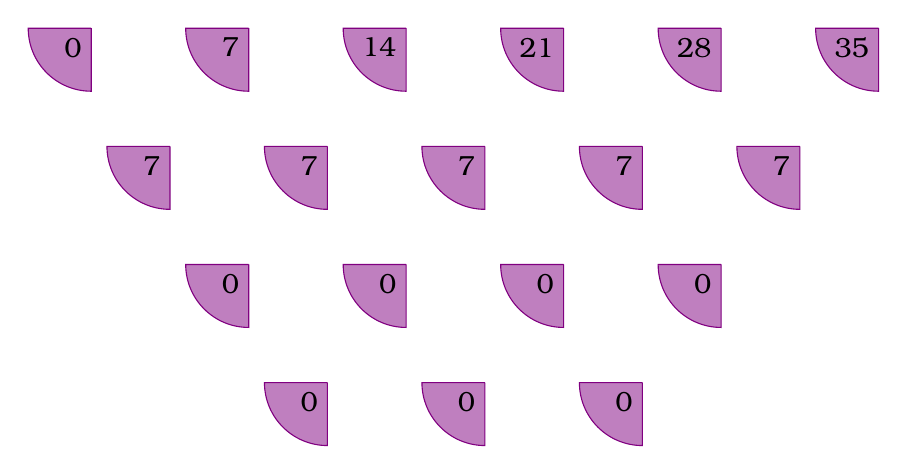
\begin{tikzpicture}[scale=1]
      
      %第三象限         
      
      \foreach \x in {0,2,4,6,8,10}  {  
      	\filldraw[fill=violet,fill opacity=0.5,draw=violet] (\x,0) -- (\x-0.8,0)
      	arc [start angle=180, end angle=270, radius=0.8]--(\x,0);
      }
      \node () at (0,0) [below left]{0};
      \node () at (2,0) [below left]{7};
      \node () at (4,0) [below left]{14};
      \node () at (6,0) [below left]{21};
      \node () at (8,0) [below left]{28};
      \node () at (10,0) [below left]{35};
      
      \foreach \x in {1,3,5,7,9}  {  
      	\filldraw[fill=violet,fill opacity=0.5,draw=violet] (\x,-1.5) -- (\x-0.8,-1.5)
      	arc [start angle=180, end angle=270, radius=0.8]--(\x,-1.5);
      	\node () at (\x,-1.5) [below left]{7};
      }
      
      
      \foreach \x in {2,4,6,8}  {  
      	\filldraw[fill=violet,fill opacity=0.5,draw=violet] (\x,-3) -- (\x-0.8,-3)
      	arc [start angle=180, end angle=270, radius=0.8]--(\x,-3); \node () at (\x,-3) [below left]{0};
      }
      
      
      \foreach \x in {3,5,7}  {  
      	\filldraw[fill=violet,fill opacity=0.5,draw=violet] (\x,-4.5) -- (\x-0.8,-4.5)
      	arc [start angle=180, end angle=270, radius=0.8]--(\x,-4.5);
      	\node () at (\x,-4.5) [below left]{0};
      }
      
      \end{tikzpicture}
  \end{frame}      


              \begin{frame}
     \frametitle{(4)差分表}
     
     \begin{tikzpicture}[scale=0.65]
     
     %第三象限         
     {\footnotesize 
     \foreach \x in {0,2,4,6,8,10}  {  
     	\filldraw[fill=violet,fill opacity=0.5,draw=violet] (\x,0) -- (\x-0.8,0)
     	arc [start angle=180, end angle=270, radius=0.8]--(\x,0);
     }
     \node () at (0,0) [below left]{0};
     \node () at (2,0) [below left]{7};
     \node () at (4,0) [below left]{14};
     \node () at (6,0) [below left]{21};
     \node () at (8,0) [below left]{28};
     \node () at (10,0) [below left]{35};
     
     \foreach \x in {1,3,5,7,9}  {  
     	\filldraw[fill=violet,fill opacity=0.5,draw=violet] (\x,-1.5) -- (\x-0.8,-1.5)
     	arc [start angle=180, end angle=270, radius=0.8]--(\x,-1.5);
     	\node () at (\x,-1.5) [below left]{7};
     }
     
     
     \foreach \x in {2,4,6,8}  {  
     	\filldraw[fill=violet,fill opacity=0.5,draw=violet] (\x,-3) -- (\x-0.8,-3)
     	arc [start angle=180, end angle=270, radius=0.8]--(\x,-3); \node () at (\x,-3) [below left]{0};
     }
     
     
     \foreach \x in {3,5,7}  {  
     	\filldraw[fill=violet,fill opacity=0.5,draw=violet] (\x,-4.5) -- (\x-0.8,-4.5)
     	arc [start angle=180, end angle=270, radius=0.8]--(\x,-4.5);
     	\node () at (\x,-4.5) [below left]{0};
     }
     
       \foreach \x in {12,14,16,18,20,22}  {  
       	\filldraw[fill=violet,fill opacity=0.5,draw=violet] (\x,0) -- (\x-0.8,0)
       	arc [start angle=180, end angle=270, radius=0.8]--(\x,0);
       }
       \node () at (12,0) [below left]{0};
       \node () at (14,0) [below left]{1};
       \node () at (16,0) [below left]{2};
       \node () at (18,0) [below left]{3};
       \node () at (20,0) [below left]{4};
       \node () at (22,0) [below left]{5};
       
       \foreach \x in {13,15,17,19,21}  {  
       	\filldraw[fill=violet,fill opacity=0.5,draw=violet] (\x,-1.5) -- (\x-0.8,-1.5)
       	arc [start angle=180, end angle=270, radius=0.8]--(\x,-1.5);
       	\node () at (\x,-1.5) [below left]{1};
       }
       
       
       \foreach \x in {14,16,18,20}  {  
       	\filldraw[fill=violet,fill opacity=0.5,draw=violet] (\x,-3) -- (\x-0.8,-3)
       	arc [start angle=180, end angle=270, radius=0.8]--(\x,-3); \node () at (\x,-3) [below left]{0};
       }
       
       
       \foreach \x in {15,17,19}  {  
       	\filldraw[fill=violet,fill opacity=0.5,draw=violet] (\x,-4.5) -- (\x-0.8,-4.5)
       	arc [start angle=180, end angle=270, radius=0.8]--(\x,-4.5);
       	\node () at (\x,-4.5) [below left]{0};
       }
  }  
        \node () at (5,-6) {{\Huge $ \times 1 $}};
       \node () at (17,-6) {{\Huge $ \times 7 $}};
       \node () at (11,-5.5) {{\Large 分拆}};
       \draw [->,line width=1pt](7,-6) --(15,-6);    

     \end{tikzpicture}
 \end{frame}      

%第四张差分表
       \begin{frame}
      \frametitle{(4)差分表}
      
      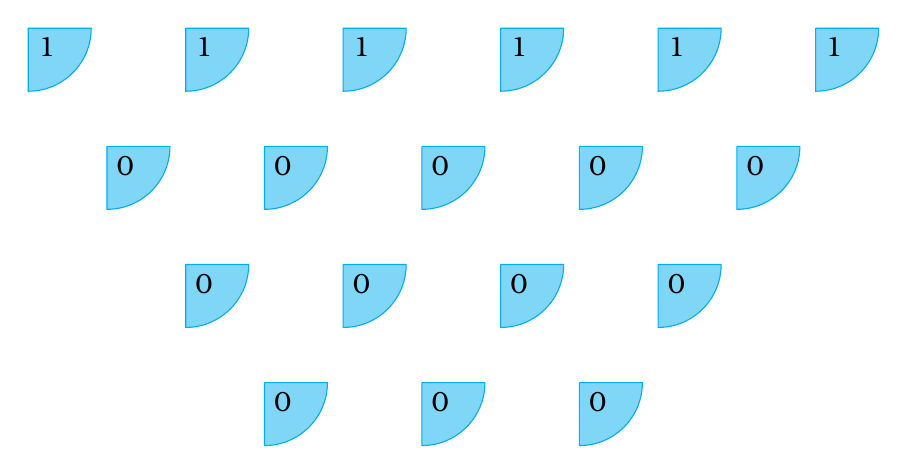
\begin{tikzpicture}[scale=1]
      
      %第四象限       	
      \foreach \x in {0,2,4,6,8,10}  {
      	\filldraw[fill=cyan,fill opacity=0.5,draw=cyan] (\x,0) -- (\x+0.8,0)
      	arc [start angle=0, end angle=-90, radius=0.8]--(\x,0);
      	\node () at (\x,0)[below right] {1};
      }
      
      \foreach \x in {1,3,5,7,9}  {
      	\filldraw[fill=cyan,fill opacity=0.5,draw=cyan] (\x,-1.5) -- (\x+0.8,-1.5)
      	arc [start angle=0, end angle=-90, radius=0.8]--(\x,-1.5);
      	\node () at (\x,-1.5)[below right] {0};
      }  
      
      
      \foreach \x in {2,4,6,8}  {
      	\filldraw[fill=cyan,fill opacity=0.5,draw=cyan] (\x,-3 )-- (\x+0.8,-3)
      	arc [start angle=0, end angle=-90, radius=0.8]--(\x,-3);
      	\node () at (\x,-3)[below right] {0};
      }
      
      \foreach \x in {3,5,7}  {
      	\filldraw[fill=cyan,fill opacity=0.5,draw=cyan] (\x,-4.5) -- (\x+0.8,-4.5)
      	arc [start angle=0, end angle=-90, radius=0.8]--(\x,-4.5);
      	\node () at (\x,-4.5)[below right] {0};
      }  
      
      \end{tikzpicture}
  \end{frame}

      \begin{frame}
      \frametitle{(4)差分表}
      
      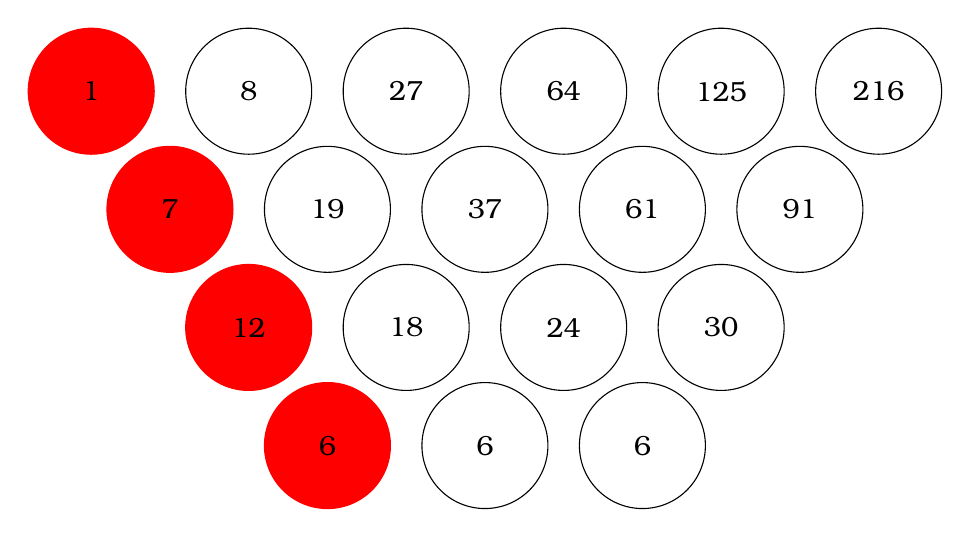
\begin{tikzpicture}[scale=1]
      \draw[fill=red,draw=red] (0,0) circle (0.8);
      \foreach \x in {2,4,6,8,10}  {
      	\draw(\x,0) circle (0.8);
      } 
      \node () at (0,0) {1};   
      \node () at (2,0) {8};
      \node () at (4,0) {27};
      \node () at (6,0) {64};
      \node () at (8,0) {125};
      \node () at (10,0) {216};
     
     \draw[fill=red,draw=red] (1,-1.5) circle (0.8); 
      \foreach \x in {3,5,7,9}  {
      	\draw (\x,-1.5) circle (0.8);
      } 
      \node () at (1,-1.5) {7};
      \node () at (3,-1.5) {19};
      \node () at (5,-1.5) {37};
      \node () at (7,-1.5) {61};
      \node () at (9,-1.5) {91};
      
      \draw [fill=red,draw=red] (2,-3) circle (0.8);
      \foreach \x in {4,6,8}  {
      	\draw (\x,-3) circle (0.8);
      } 
      \node () at (2,-3) {12};
      \node () at (4,-3) {18};
      \node () at (6,-3) {24};
      \node () at (8,-3) {30};
      
      \draw [fill=red,draw=red]  (3,-4.5) circle (0.8);
      \foreach \x in {5,7}  {
      	\draw (\x,-4.5) circle (0.8);
      } 
      \node () at (3,-4.5) {6};
      \node () at (5,-4.5) {6};
      \node () at (7,-4.5) {6};
      
      \end{tikzpicture}
  \end{frame}
      
       
       \begin{frame}
      \frametitle{(4)差分表}
      \begin{columns}
      	\column{0.48\textwidth}
      	\includegraphics[scale=0.3]{差分表.jpg}
      	\vspace{2cm}
      	\column{0.48\textwidth}
      	\includegraphics[scale=0.3]{差分算法.jpg}
      	\vspace{2cm}
      \end{columns}      
  \end{frame}

\subsection{2.在图形拼接中探究摸索}
     \begin{frame}
     \frametitle{2.在图形拼接中探究摸索}
     \begin{figure}
     	\centering
     	\includegraphics[scale=0.3]{角尺.jpg}
     \end{figure}
     \end{frame}

\subsubsection{(5)角尺拼图一}
   \begin{frame}
   \frametitle{(5)角尺拼图一、二}
        \begin{columns}
       	\column{0.48\textwidth}
       	\includegraphics[scale=0.3]{角尺拼图一.jpg}
       	
       	\column{0.48\textwidth}
       	\includegraphics[scale=0.3]{角尺拼图二.jpg}
       \end{columns}      
   \end{frame}
\subsubsection{(6)角尺拼图二}

\subsubsection{(7)旋转拼图}
       \begin{frame}
       \frametitle{(7)旋转拼图}
       \begin{columns}
       	\column{0.48\textwidth}
       	\includegraphics[scale=0.3]{旋转拼图.jpg}
       	
       	\column{0.48\textwidth}
       	\[  \sum_{k=1}^{n} k^3= \frac{\left( n\left( n+1\right) \right) ^2}{ \colorbox{red}{{\Huge 4}} } \]
       \end{columns}      
   \end{frame}

\subsubsection{(8)(割补后)三角形拼图}
       \begin{frame}
      \frametitle{(8)(割补后)三角形拼图}
      \begin{figure}
      	\centering
      	\includegraphics[scale=0.3]{三角形拼图.jpg}
      \end{figure}
  \end{frame}

\subsubsection{(9)等边三角形拼图}
        \begin{frame}
        \frametitle{(9)等边三角形拼图}
        \begin{columns}
        	\column{0.51\textwidth}
        	\includegraphics[scale=0.375]{三角形教堂屋顶.jpg}
        	
        	\column{0.48\textwidth}
        	\includegraphics[scale=0.3]{等边三角形拼图.jpg}
        \end{columns}      
    \end{frame}
\subsection{3.借助技术实现别样想法}
        \begin{frame}
      \frametitle{3.借助技术实现别样想法}
      \begin{columns}
      	\column{0.5\textwidth}
      	\includegraphics[scale=0.3]{定积分图示.jpg}
      	
      	\column{0.48\textwidth}
        \color{red} 多出一块\[   \int_{k}^{k+\frac{1}{2} } x^3 dx - \frac{k^3}{2}   \]   \\
        \color{blue!50!white} 少掉一块 \[ \frac{k^3}{2} - \int_{k-\frac{1}{2}}^{k } x^3 dx \]   \\
        \hspace{2cm}
      \end{columns}      
  \end{frame}

\subsubsection{(10)积分思想}
       \begin{frame}
       \frametitle{(10)积分思想}
       \begin{columns}
       	\column{0.33\textwidth}
       	\includegraphics[scale=0.22]{积分运算1.jpg}\\
       	\scriptsize{曲边梯形相较于矩形面积\color{red}多了$ \frac{k}{4} $}\\
       	\hspace{1cm}
       	
       	\column{0.33\textwidth}
       	\includegraphics[scale=0.22]{积分运算2.jpg}\\
       	\scriptsize {TI-Nspire的计算机代数系统(CAS)}\\
       	\hspace{1cm}
       	\column{0.33\textwidth}
       	\includegraphics[scale=0.22]{积分运算3.jpg}\\
       \scriptsize {\phantom{TI-Nspire的计算机代数系统(CAS)}}\\
       	\hspace{1cm}
       \end{columns}            
   \end{frame}

\subsubsection{(11)导数思想}
       \begin{frame}
       \frametitle{(11)导数思想}
       \begin{columns}
       	\column{0.33\textwidth}
       	\includegraphics[scale=0.22]{导数1.jpg}\\
       	\scriptsize{适当定义新函数}\\
       	\hspace{1cm}
       	
       	\column{0.33\textwidth}
       	\includegraphics[scale=0.22]{导数2.jpg}\\
       	\scriptsize {导数功能与求解方程组功能}\\
       	\hspace{1cm}
       	\column{0.33\textwidth}
       	\includegraphics[scale=0.22]{导数3.jpg}\\
       	\scriptsize {\phantom{导数功能与求解方程组功能}}\\
       	\hspace{1cm}
       \end{columns}            
   \end{frame}

\subsection{4.大胆尝试技术验证}
\begin{frame}
\frametitle{4.大胆尝试技术验证}
\begin{itemize}
	\item  运用累加化归
	\item  运用Abel变换化归
	\item  运用二项式定理化归
	\item  运用组合数性质二化归
	\item  裂项相消
\end{itemize}
\end{frame}
 
 
\begin{frame}
\frametitle{化归}
	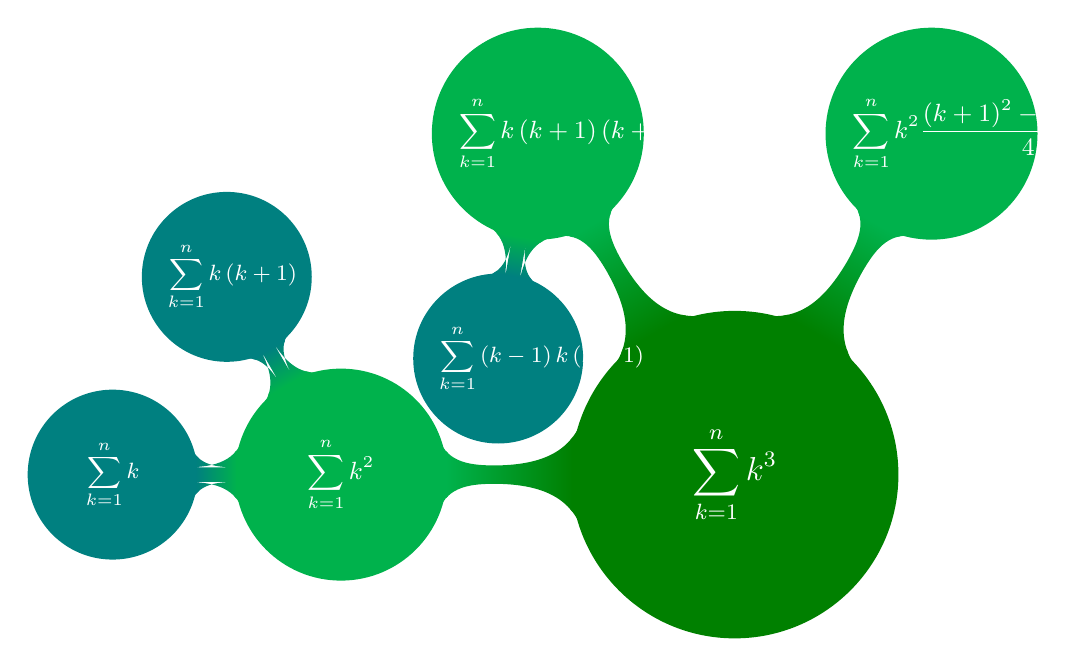
\begin{tikzpicture}[scale=1]
	\path[mindmap,concept color=green!50!black,text=white] node[concept] { \[ \sum_{k=1}^{n} k^3 \] }
	[clockwise from=180]
	child[concept color=green!70!blue,text=white] {node[concept] {\[  \sum_{k=1}^{n} k^2  \]}
		[clockwise from=180]
		child [concept color=green!50!blue] { node[concept] {\[ \sum_{k=1}^{n}  k  \]}}
		child [concept color=green!50!blue] { node[concept] {\[  \sum_{k=1}^{n} k \left( k+1\right)\ \] }}
	}
	child[concept color=green!70!blue,text=white]  {node[concept] {\[  \sum_{k=1}^{n} k\left( k+1\right) \left( k+2\right)  \]}
		[clockwise from=260]
		child [concept color=green!50!blue]{ node[concept] {\[  \sum_{k=1}^{n} \left( k-1\right) k  \left( k+1\right)  \]}}
	}
	child[concept color=green!70!blue,text=white] {node[concept] {\[  \sum_{k=1}^{n} k^2\frac{\left( k+1\right) ^2-\left( k-1\right)^2}{4}  \]}
	};
	\end{tikzpicture}

\end{frame}

\section{参考文献} 
    \begin{frame}
    \frametitle{参考文献}
  {\scriptsize  $\left[ 1 \right] $ \hspace{1em} 徐希来.中学数学课堂教学中提高记忆效能策略的研究[D].上海:华东师范大学,2018:67-71.}\\
   {\scriptsize   $ \left[ 2 \right]  $ \hspace{1em} 张礼恩.对正整数立方和公式推导的赏析[J].上海中学数学.2012,(11):43-45.}
     \end{frame}
\section{致谢}
 \begin{frame}
 \frametitle{Thank you!}
 I am reachable at xuxilai2003@163.com.\vspace{1em}
 
 \tiny The \LaTeX\hspace{0.01em} source of this presentation template is available at http://www.latexstudio.net/archives/51630.html.\\
 The template is MIT licensed.
\end{frame}
 
%\begin{frame}
%\frametitle{Title}
%This is a text from the first frame.
%\end{frame}
%\begin{frame}
%\frametitle{Image}
%\end{frame}
 
\end{document}
